\documentclass[11pt]{article}
\usepackage[letterpaper, margin = 1 in]{geometry}
\usepackage{tabularx}
%\usepackage{ltablex}
%\usepackage{tabularray}
\usepackage{array}
\usepackage{booktabs}
\usepackage{longtable}
\usepackage{caption}
\usepackage{verbatim}
\usepackage{graphicx}
%\usepackage{tblr-extras}
%\UseTblrLibrary{caption}
%\usepackage[colorlinks=true, urlcolor=blue, linkcolor=black, citecolor=blue]{hyperref}


\title{\textbf{Revision 0: \\Requirements and Hazard Analysis \\ \large Group 8 - C.A.V.E: Cave Assessment and Visualization Equipment}}
\author{Abdul Rahim Khan \\ Andrew Brink \\ Gokberk Yilmaz \\ Nicholas Trimble \\ Tabish Faisal}
\date{November 16, 2025}
%\input{../Comments}
%\input{../Common}

\begin{document}

\maketitle
%\thispagestyle{empty}

~\newpage

\pagenumbering{roman}

%	\begin{table}[hp]
%		\caption{Revision History} \label{TblRevisionHistory}
%		\begin{tabularx}{\textwidth}{llX}
%			\toprule
%			\textbf{Date} & \textbf{Developer(s)} & \textbf{Change}\\
%			\midrule
%			Date1 & Name(s) & Description of changes\\
%			Date2 & Name(s) & Description of changes\\
%			... & ... & ...\\
%			\bottomrule
%		\end{tabularx}
%	\end{table}

%\tableofcontents


\pagenumbering{arabic}

	\section{Introduction}
		This document will define the scope of the C.A.V.E. system: what inputs it collects, what processing it does, and what outputs is creates. It will define all the variables and constants used to achieve this, as well as any notation or technical terms that are needed. There will also be a fault tree analysis (FTA) breakdown of the possible root causes of failure that will inform some of the safety requirements of the system. 
		
	\section{Requirements}
	
	System Diagram 
	
	Definitions and Notation 
	
	Variables – monitored, controlled. Constants w/ nominal values. 
	
	Diagrams showing decomposition (?) 
	
	Safety/security requirements – reference hazard analysis in appendix 
	
	Requirements – required behaviour descripton, no design. Rationale, timing reqs, hardware, software, undesired event handling (safety), which are likely to change or aren’t 
	
	Very rough sketch of what is part of our system, what is not, and what the general structure of our design is (this is definitely not final, but I think it is a good start):
	
	%insert image
	\begin{figure}[h]
		\centering
		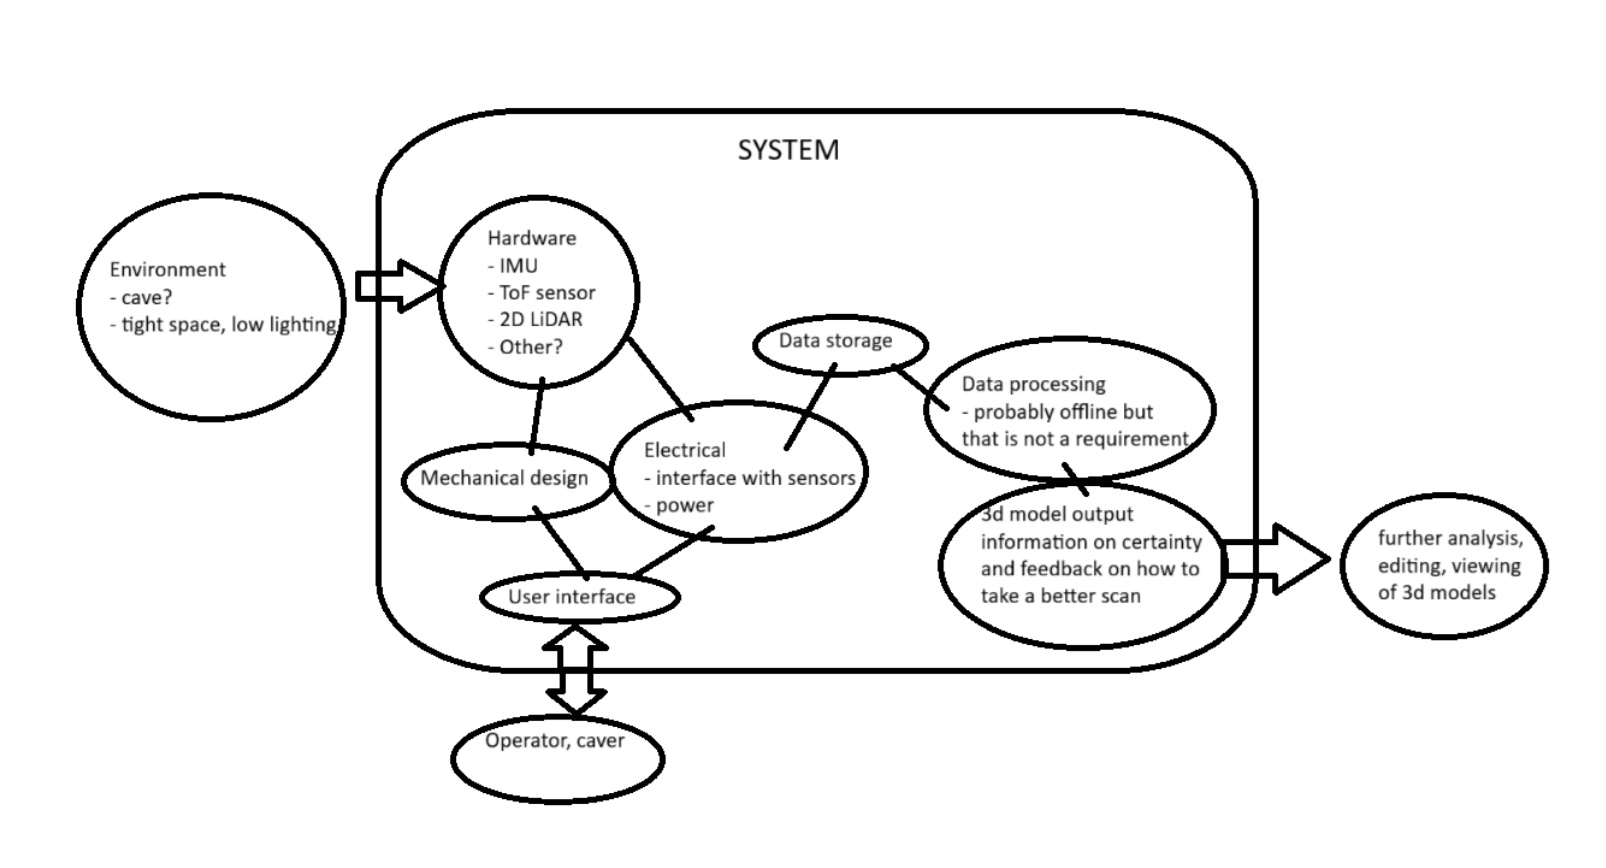
\includegraphics[width=0.9\textwidth]{images/SystemDiagram}
		\caption{General structure of the system}
	\end{figure}
	
	\textbf{Monitored variables: }
	\begin{itemize}
		\item 	M\_tof\_data: matrices of distances to objects in environment 
		\item 	M\_imu\_data: Orientation information from sensor (not sure if all the sensed values should be broken out here, if so that would be magnetometer, accelerometer, and gyroscope x, y, and z values) -going the split them to pad the report :) -Nicholas 
		\item 	M\_lidar\_data: 2D Li-DAR scan 
		\item 	M\_start\_stop: user interface button to start, stop scan  	
		\item 	M\_battery\_level: no idea if we can monitor battery levels; even if so, should this be included here? 
	\end{itemize}
		
	\subsection{Monitored and Controlled Variables}
		Monitored variables are information from the environment being input to the system, and controlled variables are the output products of the system’s internal processes. The following tables list and describe these variables in the C.A.V.E. system. 
	
		\begin{tabularx}{\textwidth}{X X X X}
			\toprule
			\textbf{Variable} & \textbf{Description} & \textbf{Unit} & \textbf{Purpose} \\
			\midrule
			M\_tof\_data & A single dot matrix frame captured from the environment  & Array of depths and positions in metres  & Capturing the contours and shape of the environment \\
			\midrule
			M\_imu\_position & Device distance from C\_START\_POSN as measured by the IMU  & Metres in (x,y,z) 
			
			!!I’m assuming the IMU measures an offset from its power on location  & Provide reference for position change between M\_tof\_data captures  \\
			\midrule
			M\_imu\_attitude & Device rotation about the x, y, z axes, measured by IMU  & Degrees: rotation from a reference frame & Provide reference for space frame rotation   \\
			\midrule
			M\_imu\_accel & Device acceleration in x, y, z, directions, measured by IMU & Metres/second\textsuperscript{2} tuple (x,y,z) & Additional frame translation reference  \\
			\midrule
			M\_imu\_magnet & Change in magnetic field  & Check how its expressed- tesla/s?  & Additional frame rotation reference \\
			\midrule
			M\_lidar & 2D Li-DAR scan of the environment & Tuple of distance in metres and angle in degrees & Long range slice of the environment to aid convergence \\
			\midrule
			M\_start\_stop & User toggle enabling or disabling the system & Boolean, true == on & Allow user control of starting and stopping a mapping session \\
			\midrule
			M\_SOC & Remaining battery percentage & \% of total charge & Estimate remaining time available for mapping \\
			\midrule
			C\_record\_status & User facing indicator to show the status of M\_start\_stop & Boolean & Inform user of the status of M\_start\_stop \\
			\midrule
			C\_record\_remain & ... & ... & ... \\
			\bottomrule
		\end{tabularx}
	\\ \\

		\textbf{Controlled variables: }
		
		\begin{itemize}
			\item C\_record\_status: user interface light indicator (stopped, recording, error, etc) 
			\item C\_record\_time: measurement (minutes?) of how long recording can continue (based on battery level and amount of storage) (I don’t know if this is something we can do with our hardware, it just seems like a good way to fluff up the controlled variables and the system requirements) 
			\item C\_point\_cloud: point cloud created by merging all the data from the recording 
			\item C\_confidence: This could be anything from a binary “success” or “failure” indicator to a more complex indicator of which parts of the map are accurate and which ones should be scanned again in more detail. We should probably specify which one it is. 
		\end{itemize}	

			\textbf{Constants:} 
			
			\begin{itemize}
				\item Transformation matrix from each sensor to the global coordinate system (based on mechanical design) 
				\item Update rate for sensors (possibly different for each sensor) 
				\item Storage capacity of recording computer 
				\item Data rate for recording 
			\end{itemize}
		
		\textbf{Requirements:}
		
		\begin{itemize}
			\item C\_point\_cloud contains a sampling of points that represent the physical surface of the environment which has been seen by the sensors (M\_tof\_data, M\_lidar\_data) while the recording is active. 
			\item The accuracy and reliability of the data contained in C\_point\_cloud must be reflected by the C\_confidence variable.
			\item C\_record\_status toggles between recording and standby when M\_start\_stop button is pressed. If there is an error which the system cannot recover from on its own, C\_record\_status goes to error status. 
			\item C\_record\_time counts down the amount of time remaining for recording, taking the minimum of the estimated battery life (inferred using M\_battery\_level) and the amount of recording time based on free device storage space and data rate of recording. 
		\end{itemize}
		
		
		\textbf{Performance timing requirements: } \\	
		Data sample rate from sensors is the only one I can think of \\
		
		\textbf{Requirements on hardware environment:} \\
		Cave proof? \\
		
		\textbf{Requirements on software environment:} \\
		...
	\section{Hazard Analysis}
		\begin{figure}[h]
			\centering
			\rotatebox{90}{
			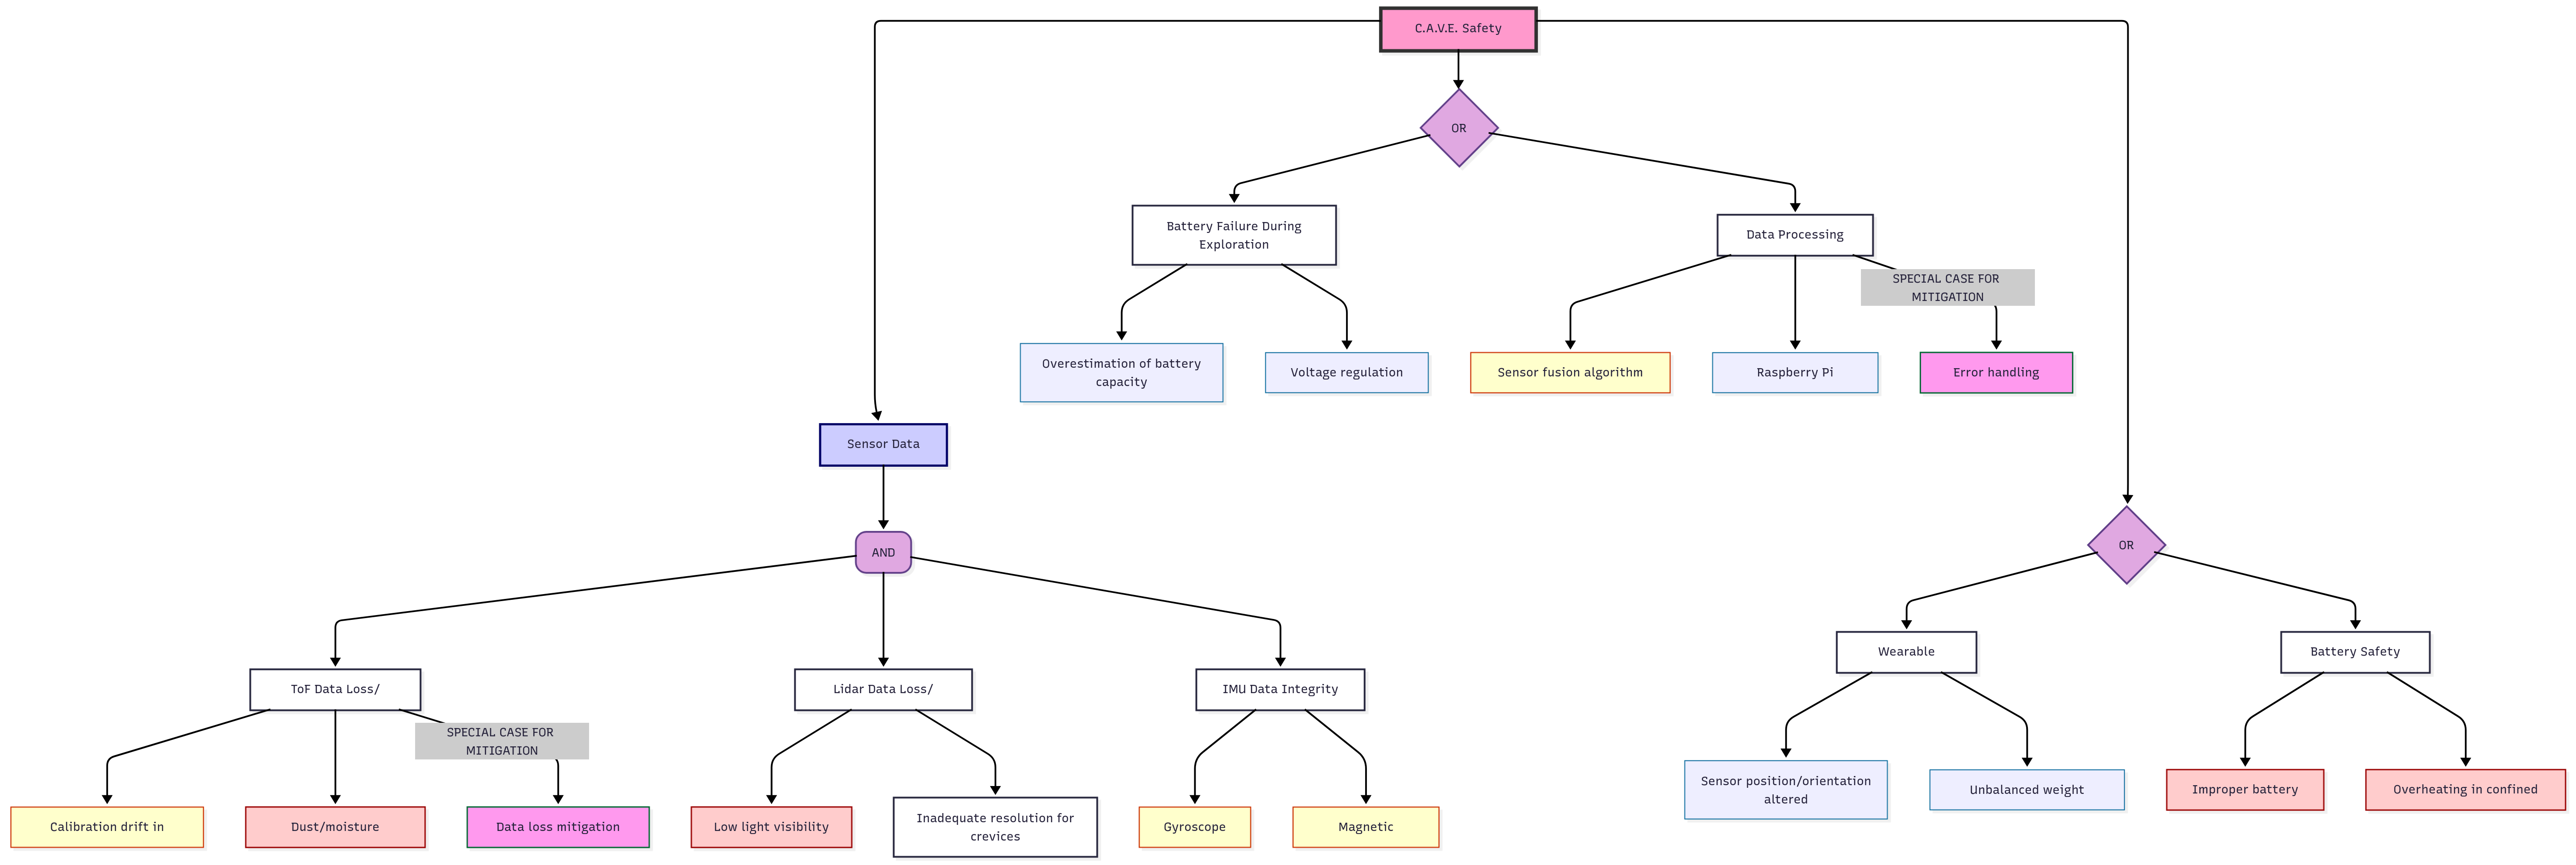
\includegraphics[width=1.35\textwidth]{images/FTA}
			}
			\caption{Fault tree analysis of the system}
		\end{figure}
		
	\begin{comment}


		
	\end{comment}



\end{document}
